%!TEX root = ../main.tex

\begin{figure}[t]
  \centering
  \begin{subfigure}{\columnwidth}
    \centering
    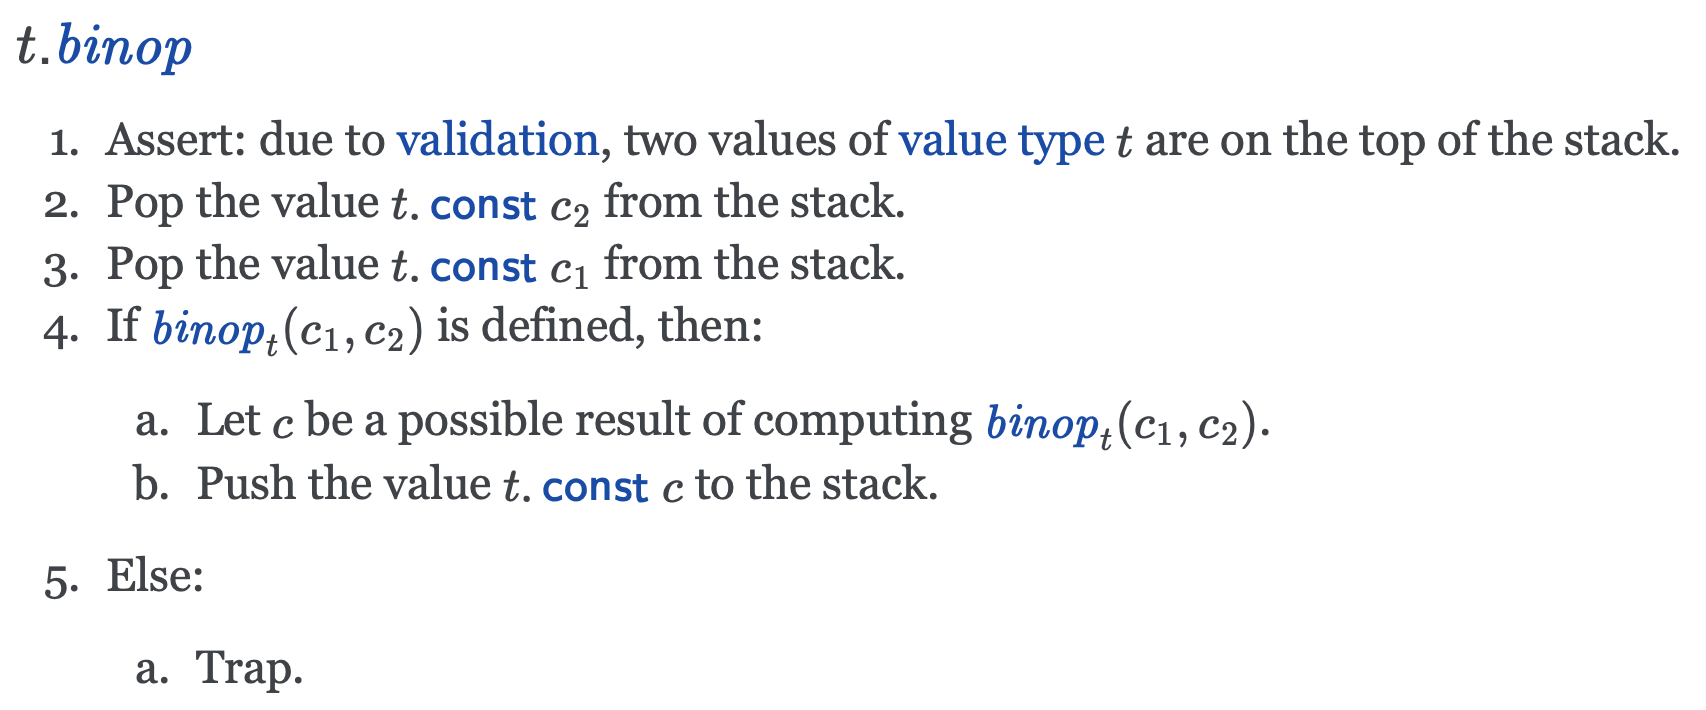
\includegraphics[width=\columnwidth]{figs/spec-prose.png}
    \subcaption{Prose specification}
\vspace*{1em}
  \end{subfigure}

  \begin{subfigure}{\columnwidth}
    \centering
    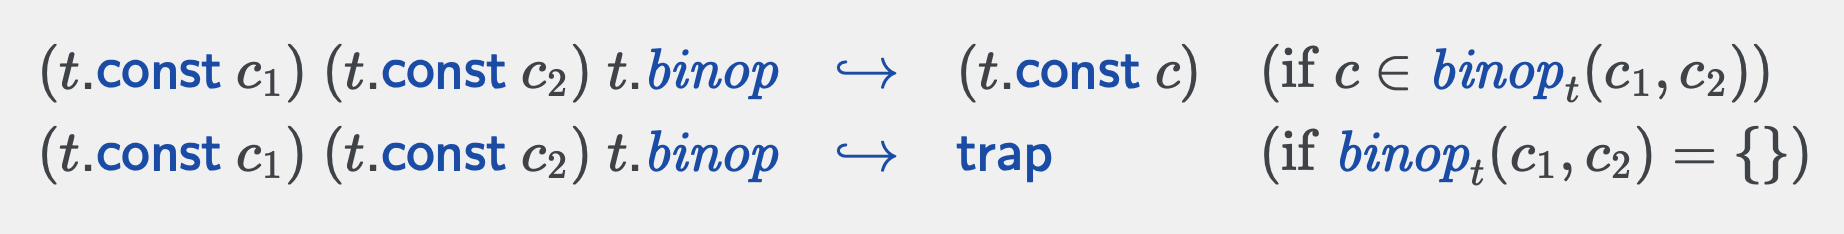
\includegraphics[width=\columnwidth]{figs/spec-formal.png}
    \subcaption{Formal specification}
  \end{subfigure}
\caption{The binary operator semantics in the specification}
\label{fig:spec}
\end{figure}

\begin{figure}[t]
\small
\begin{verbatim}
rule Step_pure/binop-val:
  (CONST nt c_1) (CONST nt c_2) (BINOP nt binop) ~> (CONST nt c)
  -- if $binop(binop, nt, c_1, c_2) = c

rule Step_pure/binop-trap:
  (CONST nt c_1) (CONST nt c_2) (BINOP nt binop) ~> TRAP
  -- if $binop(binop, nt, c_1, c_2) = epsilon
\end{verbatim}
\caption{The binary operator semantics in \dslname's DSL}
\label{fig:dsl}
\end{figure}

\begin{figure}[t]
\small
$$
\begin{array}{@{}l@{}lcl}
{[\textsc{\scriptsize E{-}binop{-}val}]} \ \
 & (\mathit{nt}.\mathsf{const}~\mathit{c}_{1})~(\mathit{nt}.\mathsf{const}~\mathit{c}_{2})~(\mathit{nt} . \mathit{binop})
 &\hookrightarrow& (\mathit{nt}.\mathsf{const}~\mathit{c}) \\
%
& \mbox{if}~{{{\mathit{binop}}{}}_{\mathit{nt}}}{(\mathit{c}_{1},\, \mathit{c}_{2})} = \mathit{c} \\
%
{[\textsc{\scriptsize E{-}binop{-}trap}]} \ \
 & (\mathit{nt}.\mathsf{const}~\mathit{c}_{1})~(\mathit{nt}.\mathsf{const}~\mathit{c}_{2})~(\mathit{nt} . \mathit{binop})
 &\hookrightarrow& \mathsf{trap} \\
%
& \mbox{if}~{{{\mathit{binop}}{}}_{\mathit{nt}}}{(\mathit{c}_{1},\, \mathit{c}_{2})} = \epsilon
\end{array}
$$
\vspace*{-1em}
\caption{The binary operator semantics in a generated PDF}
\label{fig:latex}
\end{figure}

\begin{figure}[t]
\footnotesize
\begin{verbatim}
  | binop_val  (binop : Binop_numtype) (c : C_numtype) (c_1 : C_numtype)
               (c_2 : C_numtype) (nt : Numtype) : 
    ((«$binop» (binop, nt, c_1, c_2)) == [c]) -> 
    (Step_pure ([(Admininstr.CONST (nt, c_1)),
                 (Admininstr.CONST (nt, c_2)),
                 (Admininstr.BINOP (nt, binop))],
                [(Admininstr.CONST (nt, c))]))

  | binop_trap (binop : Binop_numtype) (c_1 : C_numtype)
               (c_2 : C_numtype) (nt : Numtype) : 
    ((«$binop» (binop, nt, c_1, c_2)) == []) -> 
    (Step_pure ([(Admininstr.CONST (nt, c_1)),
                 (Admininstr.CONST (nt, c_2)),
                 (Admininstr.BINOP (nt, binop))],
                [Admininstr.TRAP]))
\end{verbatim}
\caption{The binary operator semantics in generated Lean}
\label{fig:lean}
\end{figure}